\documentclass[12pt]{report}
\usepackage{auhonors}

\usepackage{ulem}
\usepackage{url}

% % TikZ
\usepackage[latin1]{inputenc}
\usepackage{tikz} \usepackage{tkz-euclide} % loads  TikZ and tkz-base
    \usetikzlibrary{calc, arrows, shapes}
    \usetkzobj{angles} % important you want to use angles
\usepackage{pgf}


% enable expand math support
\usepackage{amsmath}
% enable graphic support
\usepackage{graphicx}

% table stuff
% \usepackage{array}
% \newcolumntype{$}{>{\global\let\currentrowstyle\relax}}
% \newcolumntype{^}{>{\currentrowstyle}}
% \newcommand{\rowstyle}[1]{\gdef\currentrowstyle{#1}%
%   #1\ignorespaces
% }

% for list of abbreviations
\usepackage[intoc]{nomencl}
\renewcommand{\nomname}{ \sc List of Abbreviations}
\makenomenclature
%% don't forget to run:   makeindex ausample.nlo -s nomencl.ist -o ausample.nls


% click on links to jump in pdf - should come last of usepackages
\usepackage{hyperref}
\hypersetup{}

% May want theorems numbered by chapter
% \newtheorem{theorem}{Theorem}[chapter]

\title{A Visual Driver Aid for Convoy Following Based on Dynamic Base Real-Time Kinematic Positioning}
\author{Robert Grissom Cofield}
\date{May 5, 2013}
\copyrightyear{2013}
\adviser{David M. Bevly}

\professor{David M. Bevly \\ Professor \\ Mechanical Engineering}
\professor{Constance C. Relihan \\ Associate Provost for \\ Undergraduate Studies}


\begin{document}


% TikZ styles
% Define block styles
\tikzstyle{decision} = [diamond, draw, fill=blue!20, text width=4.5em, text badly centered, node distance=3cm, inner sep=0pt]
\tikzstyle{block} = [rectangle, draw, fill=blue!20, text width=5em, text centered, rounded corners, minimum height=4em]
\tikzstyle{line} = [draw, -latex']
\tikzstyle{cloud} = [draw, ellipse,fill=red!20, node distance=3cm, minimum height=2em]



%%%%%%%%%%%%%%%%%%%%%%%%%%%%%%%%%%%%%%%%%%%%%%%%%%%%%%%%%%%%%%%%%%%%%%%%%%%%%%%%
%   Prefatory Pages
%%%%%%%%%%%%%%%%%%%%%%%%%%%%%%%%%%%%%%%%%%%%%%%%%%%%%%%%%%%%%%%%%%%%%%%%%%%%%%%%

\begin{romanpages}

\ApprovalPage
\TitlePage
\CopyrightPage

\begin{vita}%\def\romanpages{0}
Robert Cofield ...
\end{vita}


\begin{abstract}
Abstract goes here ...
\end{abstract}


\begin{acknowledgments}
Thank people here ...
\end{acknowledgments}


\style{ASME}
\software{
    cProfiler,
    Google Earth v7.0.3.8542,
    \LaTeX, TikZ, 
    MATLAB v7
    Matplotlib,
    MOOS v10,
    NumPy,
    Parallels, 
    pyMOOS,
    PySide v1.1.1,
    Python v2.7.3,
    Qt v4.8.3,
    Qt4 Designer,
    SciPy,
    Sublime Text 2,  
    simplekml v1.2.1,
    Tornado v2.3,
}
\StylePage

\tableofcontents
\listoffigures
\listoftables

\printnomenclature[0.75in] 

\end{romanpages}

\normalem       % Make italics the default for \em


%%%%%%%%%%%%%%%%%%%%%%%%%%%%%%%%%%%%%%%%%%%%%%%%%%%%%%%%%%%%%%%%%%%%%%%%%%%%%%%%
%   Chapter 1
%%%%%%%%%%%%%%%%%%%%%%%%%%%%%%%%%%%%%%%%%%%%%%%%%%%%%%%%%%%%%%%%%%%%%%%%%%%%%%%%
\chapter{Introduction}

% Establish the use case
The convoy scenario is examined, wherein a chain of vehicles are aligned front to back along some path determined by the front-most vehicle. Each inner vehicle acts as a leader to that following it, and follows the one preceding it. As such, vehicle must maintain some form of communication with those directly adjacent to it. The computational tasks for each leader-follower pairing is carried out in the following vehicle. This is typically done in the lead vehicle for other secenarios, such as when the follower is an unmanned aerial vehicle, as UAV's are often limited by weight, and thus outsource processing tasks to ground computers where possible. Relying on the leader for positioning data is even used for swarm setups with a single leader and multiple followers \cite{gian}, regardless of the positioning method. For the present scenario, however, this structure makes the implementation of visualization software for data recieved from each leader much easier to implement with a low computational cost. The following chapter highlights why a navigational aid is necessary for convoy scenarios, why DRTK with TDCP is the ideal solution, and how it functions.

\section{Motivation} %% GET CITATIONS!
%Autonomous scenarios?
% military convoys
The military often uses long trains of transport vehicles to move supplies and munitions through perilous terrain over long distances. Landmines and other explosive roadside devices are common in many combat environments, and a precise path of safe travel may be defined. Rather than use at least one soldier to operate each vehicle, having a single human driver in the lead would reduce manpower and, potentially, casualties in the event that a convoy is attacked. In addition, a machine-driven following vehicle can potentially acheive much greater lateral path following accuracy than a human-driven vehicle.

% commercial trucking
Commercial trucking accounts for XXXXX of all vehicles on the road. In areas where traffic congestion is a serious problem, automation of the driving task could allow for tighter truck groupings, easing congestion and avoiding vehicular collisions. When extremely close together, vehicles experience the aerodynamic phenomenon known as `drafting', whereby the air drag created by a lead vehicle clears the way for those following it, thereby lessening the total force required to propel the vehicle and significantly lowering fuel consumption. In addition, driver `down time'---when truck drivers must rest periodically and stop the vehicle---could almost be eliminated by placing drivers in two to three trucks and having them take turns as the leader of the convoy, resting and allowing the automated following system to control their truck. This would also drastically reduce the labor required to move goods via the highway system

%%%%%%%%%%%%%%%%%%%
% COMPARE SOLUTIONS
\section{Comparison of Positioning Solutions for Real-Time Following}
An abundance of alternatives exist for positioning one vehicle behind another. Many incorporate fusion algorithms, wherein data from multiple sensors providing the same information is intelligently assigned varying weights in the determination of an overall solution. In addition, coupling sensors with complimentary strengths (e.g., IMU and GPS) has proven to be an extremely robust and effective method of localization and navigation \cite{scottthesis}. The following section will overview the strengths and weaknesses of each as a standalone sensor employed for vehicular following as compared DRTK/TDCP.

%%%% RANGING
\subsection{Ranging Devices}
Ranging devices operate on a similar principle to GPS pseudoranging, i.e., time-of-flight. A signal of some type is emitted from the ranging instrument and reflected off some object. Many of the signals return to the ranging device, whereupon the elapsed time is multiplied by the speed of the signal to yield a range. These all require that the object detected be visible to the instrument, or have a direct line of sight. While useful in many situations, the present scenario does not always provide for direct line of sight, such as when a leading vehicle rounds a corner or sharp curve.

% RADAR - finished
The most popular of these technologies is Radio Dectection and Ranging (RADAR), which came to prominence during WWII, and is widely used for adaptive cruise control (ACC) in the automotive industry. The scenario of ACC is similar to the present scenario in that relative positioning is employed to monitor the location of a vehicle travelling directly ahead along a comparable path. The primary goal is to sustain a target forward velocity until doing so would result in a rear-end collision.  RADAR is capable of detecting the kinematic movement of multiple objects within its field of view, but must maintain line-of-sight \cite{lidarvsradaracc}. This does well for avoidance scenarios, but the present objective---while avoiding a rear-end collision is desirable---is quite the opposite.

% SONAR - finished
The simplest implementation of this concept is Sonic Navigation and Ranging (SONAR). Sound waves are emitted and upon return, the calculated distance indicates an object at the determined range somewhere within the field of the emitter. As this provides no orientation, arrays of SONAR devices must often be used to successfully avoid obstacles. This may be combined with odometry to some effect, but navigation is very difficult and highly imprecise.

% LiDAR - finished
Light Detection and Ranging (LiDAR) allows measurement of not only a very precise position, but the optical properties of the detected object. A beam of light is emitted and reflected back to the instrument, whereupon the elapsed time is multiplied by the speed of light to yield a range. For relative positions to be accurate, either mounting of the instrument must be extremely precise or a calibration process is required \cite{jordanlidar}. Once properly tuned, LiDAR may produce errant readings during inclement weather, and also necessitates the adjacent leader to be within line-of-sight for any useable data to be returned. On the other hand, LiDAR also yields a numerical value for the intensity of the objects which are visible, which can be used to determine lateral path deviation provided that lane markings are visible and the path lies within them \cite{cameralidarlane}. 

%%%% VISION
\subsection{Vision}
Convoy following algorithms based on computer vision has existed for quite some time \cite{visionrec}, and like LiDAR lends itself to lane-level positioning, but requires a line-of-sight for any data on the intended leader. Camera systems are also susceptible to direct sunlight, rain, and poor illumination, which in many cases render the system useless. The use of a graphics processing unit is often required, as image processing tasks are computationally expensive, sometimes prohibitively so for embedded systems.
% Mono Camera
A monocular camera employed for the present purposes will typically extract notable features from a rectangular image. To make determination of the leader's pose less error-prone, an easily extractable object of known shape and dimensions can be placed on the rear of the vehicle where it can be seen by the follower camera.
% Stereo Camera
Stereo cameras function much like the human eye, in that depth is obtained from comparing differences between two images of the same object taken simultaneously from two cameras of aligned in parallel at a known separation in the direction perpendicular to the line-of-sight.


%%%%%%%%%%%%%%
% Explain GNSS
\section{Global Navigation Satellite System}

% \subsection{Principles of GNSS}
At the fundamental level, GNSS
\footnote{GNSS is a protocol-agnostic term referring to any of several constellations worldwide which use satellites to provide a receiver on the ground with position, velocity, and time information. The US implementation is known as GPS, the Russian positioning system is referred to as GLONASS, and the European Union has Galileo.}
comprises a constellation of orbitting satellites whose positions above the earth are known, corresponding with a receiver to give as many range measurements as possible so that a global 3 dimensional location may be calculated. GNSS does not necessitate line of sight between vehicles, and is not impaired by lighting effects, though a clear view of the sky is needed to maintain data reception from as many satellites as possible. The range for highly accurate following is large, on the order of kilometers depending upon speed, and lower accuracy following can be performed for two vehicles at any distance. These make GNSS ideal for use in the leader-follower convoy scenario.

% Improvements to standalone
% RTK - finished
However, sub-meter positioning accuracy is often necessary for convoy following, and several improvements to standalone GNSS exist to acheive this accuracy. When working in a defined area, the exact location of a nearby point is known. If this is not the case, the exact location of a point may be found by setting up a static GPS receiver and allowing the measurements to average towards zero error over a long period of time. Once the precise location is known, the base station can transmit the difference between this value and the position received by standalone GPS to nearby receivers in real-time. Using these corrections to compensate for errors is known as Real Time Kinematic (RTK) GPS. It produces extremely accurate global positioning (i.e., in the earth coordinate frame).
% DRTK
RTK assumes that two receivers will experience similar errors when in close proximity and measuring simultaneously. The same principal applies to two receivers when both are kinematically active, but a globally accurate position is no longer possible without some reference. Instead, a high-accuracy relative position vector (RPV) can be obtained by subtracting the position of one receiver from that another at the same time epoch.
% TDCP
This practice of subtracting errors can be extended to work with a single receiver. Between very successive measurement epochs taken in short periods, many of the errors in standard GPS remain constant. The corresponding time difference of the carrier phase (TDCP) can then be used to calculate a change in position between time steps, also known as odometry \cite{travisdiss}.


%%%%%%%%%%%%%%%%%%%%%%%%%%%%%%%%%
% How we get what's on the screen
\section{Position Using the DRTK and TDCP Algorithms}
Figure \ref{fig:drtktdcp} illustrates how information is taken from each receiver to obtain the information necessary for the display. The algorithms used to calculate information displayed by the GUI have been developed extensively by \cite{scottthesis},\cite{travisshort}, \cite{travisconvoy} and \cite{travisdiss}. The Driver Assisted Following (DAF) algorithm adds odometry from the TDCP algorithm to RPVs from the DRTK algorithm to obtain a set of points in the East-North-Up (ENU) coordinate frame---with the origin at the follower---which lie along the path taken by the leader. Distance between relative path points depends upon the velocity of the leader and the frequency of the slowest algorithm. The specifications of all hardware used are outlined in Chapter \ref{chap:exper}.

% flowchart - How the data gets from receiver to gui
\begin{figure}[ht] \caption{Relative path determination processes} \centering \label{fig:drtktdcp}
    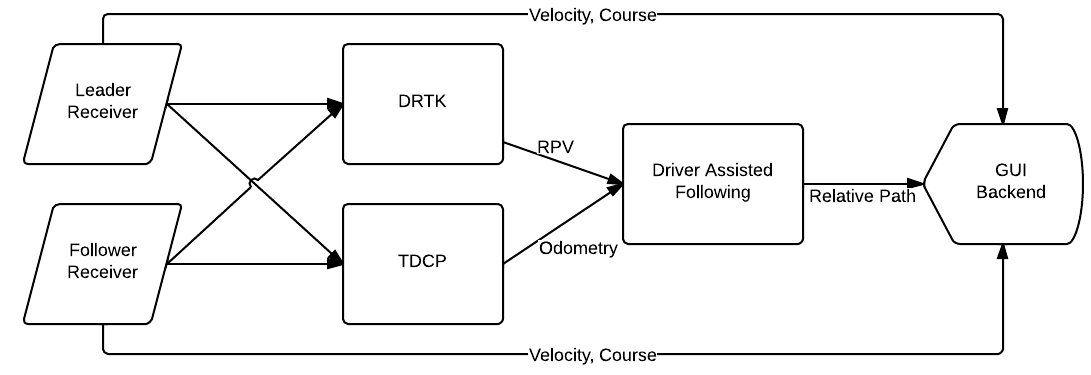
\includegraphics[width=6.5in]{./figs/data_algo.png}
\end{figure}

% DRTK accuracy - finished
The availability of DRTK GPS is primarily contingent upon the availability of dual-band (L1 and L2, rather than L1 only) signals, and of high precision ambiguity estimates (fixed integer rather than floating point). Under ideal conditions, the root-mean-square error of DRTK positions will be as low as $0.33~cm$ with a variance of $0.10~cm^2$. 
% TDCP accuracy 
The accuracy of the TDCP algorithm decreases over time as errors in the position changes accumulate. The mean time for a static receiver to accumulate $1.0~m$ lateral error is $378~s$, so the curvilinear distance at which this error will be present is contingent upon the speed of the follower. A complete analysis of the DRTK/TDCP algorithm error behavior is provided by \cite{scottthesis}.
% remove if not doing err prop
The combined accuracy traits of the system when employed for convoys of three or more vehicles are explored in Chapter \ref{chap:errprop}.
% Combined output of TDCP and DRTK for path

% Velocity accuracy





%%%%%%%%%%%%%%%%%%%%%%%%%%%%%%%%%%%%%%%%%%%%%%%%%%%%%%%%%%%%%%%%%%%%%%%%%%%%%%%%
%   Chapter 2
%%%%%%%%%%%%%%%%%%%%%%%%%%%%%%%%%%%%%%%%%%%%%%%%%%%%%%%%%%%%%%%%%%%%%%%%%%%%%%%%
\chapter{Graphical User Interface} \label{chap:gui}

%%%%%%%%%%%%%%
% Introduction
\section{Introduction} \label{sec:guiintro}

%%%% Role of the GUI
Before beginning creation of the GUI, a very high level analysis of its role was performed---it was treated as a `black box' system to define inputs and outputs. Neighboring systems which provide input to the GUI are the GPS receivers and the DAF application, and output from the GUI is sent directly to a display device. In order to robustly communicate with the input systems, a single middleware application (described in Sec. \ref{sec:datadiss}) was designed to eliminate unnecessary or redundant data transfer. The result of this `black box' analysis is the information flow architecture depicted in Fig. \ref{fig:blackboxflow}.

% list the output data: dst, dev magnitude and direction
The fundamental purpose of this graphical tool is to show a driver the path which another vehicle has taken, and how to replicate it. So a series of dicrete position goals must be displayed in some manner or frame of reference that is instantly understandable. When the position of the vehicle attempting to follow this path does not coincide with some part of that path, the driver will need to know how large the discrepancy is and how to correct it. Lastly, when visual following becomes unreliable, the risk of rear-end collision is increased, so a follower will need to know how far away the are from the vehicle in front of them and whether this distance is safe. So the GUI will show a relative path, lateral deviation from that path, and curvilinear separation (distance along the path between leader and follower) with a corresponding safety estimate.
% list the input data: pos, vel, crs, path
The inputs necessary to relay that information were then determined to be, at a minimum, the array of two dimensional path points rotated and translated into the following vehicle's coordinated frame, and velocity state of the following vehicle. Later, as development progressed to the state described in Sec. \ref{sec:finaldes_earth}, other inputs were channelled in to augment a following driver's situational awareness further.

% Black box info flow chart
\begin{figure}[ht] \caption{High level information flow architecture in and out of the GUI} \centering \label{fig:blackboxflow}
    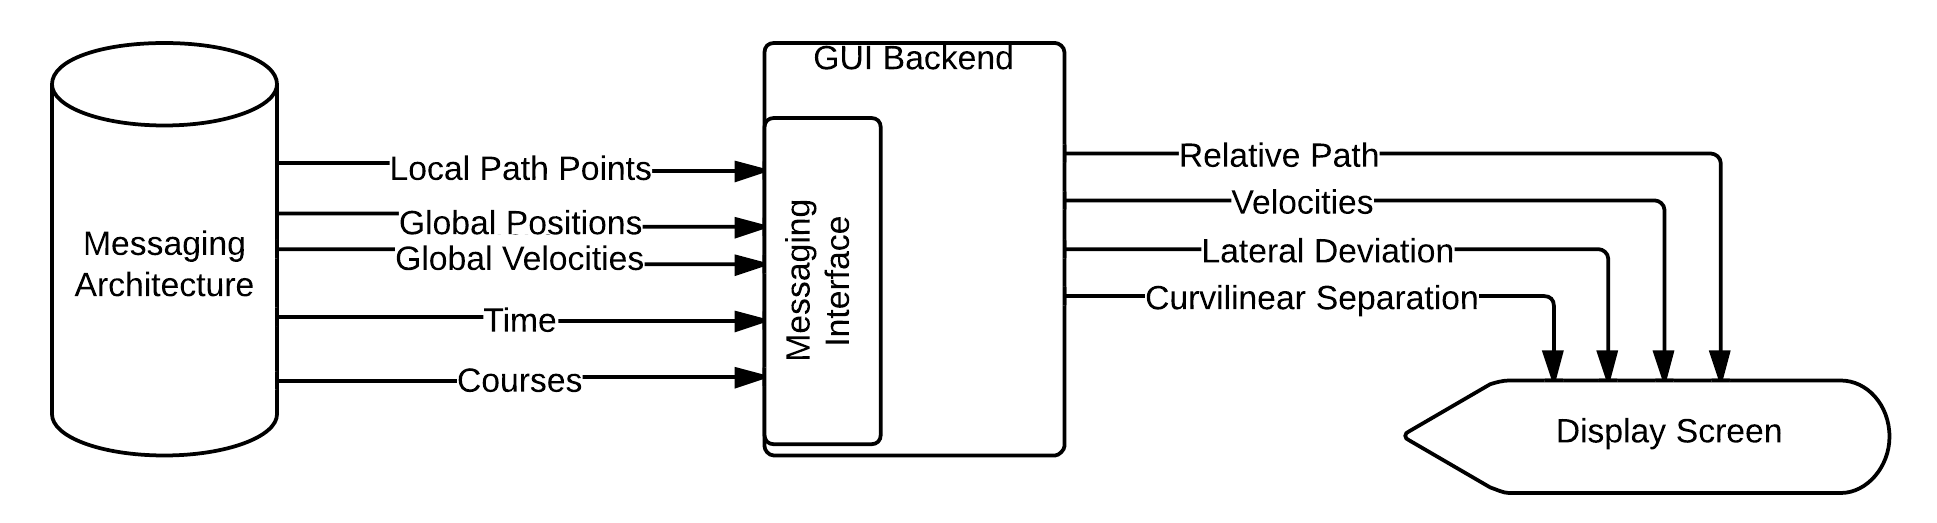
\includegraphics[width=6.5in]{./figs/blackbox_flowchart.png}
\end{figure}

% warn and crit states
When characterizing the statuses of deviation and forward distance, it was determined that a scheme similar to that of U.S. stoplights would be used in order to communicate alerts in a fashion familiar to many drivers; green denotes acceptable conditions, yellow is displayed when warning is merited, and red when a critical boundary has been violated. This coloring is used on the representation of both vehicles to relay two pieces of information: follower color indicates the corresponding value of lateral deviation relative to deviation thresholds, and leader color indicates the corresponding value of forward curvilinear separation distance relative to safe following distance thresholds. The process for determining the exact values for thresholds at which color changes occur is outlined in Sec. \ref{sec:guicalc}.

%%%% Made 2 GUIs
%% Monolith
From the outset, a primary design goal was to minimize the amount of visual and cognitive effort required on the part of the driver for determining whether course and speed corrections are necessary, and if so, what they are. Facilities for accepting driver-input operational parameters must therefore be obscured during the driving task, yet easily accessible on the fly. In addition, a clean and minimal visual presence ensures that a passing glance is sufficient to check on distance and deviations. When following very closely, a follower will need to anticipate upcoming turns without being able to see the leader actually turn, so course information---specifically, the leader's course relative to that of the follower---will be needed.  These were the fundamentals driving the GUI development at the outset. Since the resulting interface was presented in a single window on the display device and utilized only the Qt4 C++ library and associated Python bindings for rendering, it is referred to as `monolithic'.

%% Earth
Since a significant end use case involves military convoys, feedback was sought from personnel in the Armed Forces. One primary criticism was the lack of visual stimuli by which to reconcile the screen output with what the user sees around them. In essence, it was suggested, users must develop a trust with any tool before beginning to make decisions based upon it, particularly in the dire situations for which this tool is designed. To remedy this, it was proposed that satellite imagery be incorporated into the background of the information already displayed on the screen. As this directly contradicted the clean, distraction-free nature of the prototype already developed, it was determined that another version needed to be constructed following these new design principals, and that the two GUI's should be juxtaposed the most prudent approach. In determining what software package to use as an imagery backend, a trade study was performed and the resulting candidates were narrowed to Quantum GIS and Earth (by Google). The maturity, user-base and documentation on representing data with the Keyhole Markup Language (KML) ultimately made Google Earth the favored tool.

%%%%%%%%%%%%%%%%%%%%%%X
% Interpolator Section
\section{Real-Time Interpolation} \label{sec:interp}
%%%%% introductory
The addition of satellite imagery made the user highly aware of the update rate of each piece of information displayed spatially, necessitating the incorporation of data smoothing techniques. Since the end goal is to display information that has been received rather than predict future states, a minimum of two most recent data points is required to do a live interpolation. With this, a continuous-time linear interpolation of the measurement at any instant between those two times is possible. By making more data points available and considering the type or nature of data in question, more accurate form of interpolation may be possible. However, due to speed and efficiency, the linear interpolation is preferable in this situation. All values which are displayed in the GUI (listed in Sec. \ref{sec:guiintro}) are passed through the interpolation algorithm.
%%%%% general algorithm
Equation \eqref{eq:interp} gives general form of the linear interpolation to obtain a value $x$ at time $t$ which lies between values $x_0$ and $x_1$ corresponding to times $t_0$ and $t_1$, respectively.
%% formula
\begin{align} \label{eq:interp}
    x(t) &= (x_1 - x_0) \frac{ t - t_0 } { t_1 - t_0 } + x_0
\end{align}

%%%% data-type specific
For two dimensional positions, this procedure is carried out on both the East and North coordinates. 
%% angle
Angles are a different matter. The course dimension contains an inherent discontinuity due to `wrapping' at the North axis. A course change of $-1^\circ$ may result in a measurement change of $-359^\circ$, which if naively interpolated would result in a complete spin over a full timestep, ending at essentially the same location as the beginning. For this reason, the angles must be occasionally be resolved (i.e., when $|x_1 - x_0| > 180^\circ$ ) by adding $360^\circ$ to the lowest value. For example, values of $(x_0, x_1) = (0.5^\circ, 359.5^\circ)$ would then become $(x_0, x_1) = (360.5^\circ, 359.5^\circ)$ .  This value is then checked and corrected by the display controller upon rendering.
%% path
For the path to be interpolated,  the same procedure for positions is carried out for each point in the vector. A problem arises when interpolating between timesteps with unequal numbers of points, as each point cannot then be interpolated as if it were travelling along a line. When path length mismatch occurs between two successive updates, redundant points are added coincident with the rearmost path point until the two vectors are equal in length. When the number of points is decreasing, this alone would lead to a buildup of unnecessary data points, tying up valuable memory space and processing time. Thus, each time the length decreases and stays constant or continues decreasing for two or more timesteps, redundant points are removed from the saved vector.

%% time update
While GNSS provides the ability to precisely synchronize systems, display smoothing must rely upon computer-specific timestamps as some machines will operate more slowly than others. Accordingly, when initial measurement messages arrive, the CPU time at which the content of each message packet was extracted is stored along with that content. It is important that CPU time is recorded upon extraction rather than upon completion of processing or transmission, as the goal of this process is to obscure lags incurred during calculation or radio transmission; the extraction (and assignment) time represents the earliest point when any portion of the rest of the GUI may then access that data to display it. The end result is that the user is presented with data which will change at a consistent frequency (as specified by the user), regardless of whether multiple sensors take varying amounts of time to relay or calculate data.

Upon each subsequent measurement update, the two previously newest values $(x_1,t_1)$ are moved to variables for old data $(x_0, t_0)$ and the new value is stored along with present CPU time. An interpolation object representing Eq. \eqref{eq:interp} is created with the present data so that between times $t_0$ and $t_1$ an input $t$ will yield the respective measurement $x$. Any interpolation thread which is still running is then stopped, and a new one spawned. This thread begins incrementally calculating data between $x_0$ and $x_1$, then waits a period of time corresponding to the desired frequency, repeating until either a new measurement update occurs or time $t_1$ is reached.

%%%%% transition to data dissemanation
The effect this had upon readability and being able to intuitively interpret data was positive. Even though it was initially intended to smooth movement of satellite imagery and low sensor frequencies, it became desirable to investigate the benefits on the monolithic GUI. Rather than rewrite the smoothing tool for that purpose, it was modularized as described in Sec. \ref{sec:datadiss}, to distribute data agnostically.

%%%%%%%%%%%%%%%%%%%%
% Data Dissemenation
\section{Data Dissemenation} \label{sec:datadiss}

Both the GPS receivers and 
%%%% Qt Signals/Slots - REDO
The Qt \cite{qt} framework used to generate the GUI from common building blocks has an internal message passing scheme similar to a publisher/subscriber model, using instead what are called signals and slots. For instance, the main window widget alerts the render area to the left when a spinbox in the options has been changed via a signal/slot by passing a boolean value. All data coming into the GUI from MOOS passes through an interface that bridges the two with a respective signal/slot pair. In this way GUI inputs can be made agnostic to the middleware used, requiring only a simple widget be written in order to be hooked up to a new data stream. Each of these signal and slot connections are made at runtime, when the object instances to which they belong are created.

%%%% MOOS Messages - input to GUI
Figure \ref{fig:blackboxflow} depicts the predefined inputs and outputs of the GUI. The primary message passing architecture used to deliver data to the GUI, as depicted in Fig. \ref{fig:blackboxflow}, was the Mission Oriented Operating Suite (MOOS), as developed by \cite{moos}. The GUI was initially developed using postprocessed data collected from an Prowler ATV automously following an Infiniti G35 using the same positioning and radio setup described in Sect. \ref{sec:hardware}. This is made possible by the playback feature of the MOOS framework, which is used in live operation to send raw data between the GPS receiver and the DRTK, TDCP and DAF algorithms, and then to the GUI middleware interface.

%%%% Specific to Earth GUI
%% KML server
Every detail displayed in the Earth GUI at any instant is defined using the a document written in the Keyhole Markup Language. These documents must be generated at whatever screen refresh rate is desired. Supplying KML documents updating in excess of 10 Hz required contsruction of a local server which was built using the Tornado web framework. Each KML document contains 3D view information supplied by the controls located in a view tab located in the command interface described in Sec. \ref{sec:finaldes_earth}. The object which is controlled is a virtual camera perspective above the satellite imagery specified by a point of focus on which to center the screen (determined by a combination of vehicle positions), altitude above that point, tilt from vertical, and heading relative to north.
%% passing middleware object instance references
All this information is easily accessible in a central location by creating a single information object. A reference to this instance is passed to all applications which need to either update it with new data or retrieve a snapshot of the latest data from it. In this manner, creation of alternative middleware interfaces is greatly simplified.

%%%%%%%%%%%%%%
% Calculations
\section{Calculations} \label{sec:guicalc}

% UTM coordinates - REDO
When displaying data on a rectangular screen, it becomes desirable to utilize a coordinate system more suited to cartesian calculations than Latitude-Longitude-Altitude (LLA), one which employs standard metric units of length. Whenever rectangular coordinates are necessary the Universal Transverse Mercator (UTM) east and north representations of global positions are used. The conversions between the LLA and UTM coordinate systems are outlined in \cite{projections}.

%%%% Calculating the lateral error
The most crucial calculations are performed upon the vector of relative path points, of which two particular points are the subject of great attention. In Fig. \ref{fig:pathpts} the point $(x_1,y_1)$ represents the nearest (i.e., lowest distance to the origin) which also lies behind the antenna of following vehicle, meaning the vector from the origin and the follower's velocity vector form an obtuse angle. The DAF algorithm sorts and outputs points such that this will be the last in the vector, and prior to this will be the nearest point in front of the vehicle's antenna, named $(x_2,y_2)$ in Fig. \ref{fig:pathpts}. The path is assumed to be straight between these two points. The lateral deviation of a follower at $(x_0, y_0)$ from the path occurs here and is defined as the length of a line perpendicular to the path line, which it intersects at $(x_3,y_3)$---used later for forward spacing calculation. Note that depending on path shape and timing, $(x_3,y_3)$ may not necessarily lie between $(x_1,y_1)$ and $(x_2,y_2)$. Since the DAF algorithm will output in East-North coordinates translated to the follower's position, $(x_0, y_0)=(0,0)$ at all times. The formulation of the lateral deviation is then given by Eq. \eqref{eq:laterr} \cite{laterrformula}. 
% Lateral error formula
\begin{align} \label{eq:laterr}
    e &= \frac{ | (x_2 - x_1)(y_1 - y_0) - (x_1 - x_0)(y_2 - y_1) | } { \sqrt{ (x_2 - x_1)^2 + (y_2 - y_1)^2 } }
\end{align}
The underlying assumption here is that the GPS antenna is placed on the lateral center of the vehicle. Once this value has been determined, it may simply be compared against user-input threshold values for warning and critical states to determine whether to issue an alert as discussed in Secs. \ref{sec:finaldes_monolith} and \ref{sec:finaldes_earth}.

% RPV diagram
\begin{figure}[ht] \centering
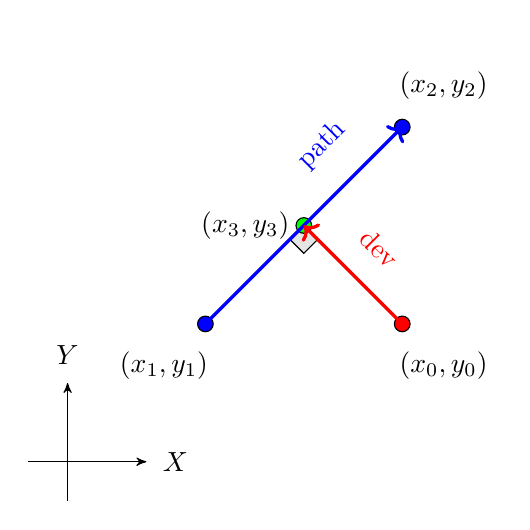
\begin{tikzpicture}[
        scale=5,
        axis/.style={thin, ->, >=stealth'},
        every node/.style={circle, color=black}   ]
    % axis
    \draw[axis] (-0.1,0) -- (0.2,0) node(xline)[right] {$X$};
    \draw[axis] (0,-0.1) -- (0,0.2) node(yline)[above] {$Y$};
    % points
    \coordinate (a) at (0.35,0.35);
    \coordinate (b) at (0.6,0.6);
    \coordinate (c) at (0.85,0.85);
    \coordinate (d) at (0.85,0.35);
    % right angle
    \tkzMarkRightAngle[fill=gray!20,size=.05](a,b,d)
    \node[draw,circle,inner sep=2pt,fill=blue] at (a) {};
    \node[draw,circle,inner sep=2pt,fill=green] at (b) {};
    \node[draw,circle,inner sep=2pt,fill=blue] at (c) {};
    \node[draw,circle,inner sep=2pt,fill=red] at (d) {};
    % point labels
    \node [below left] at (a)  {$(x_1,y_1)$};
    \node [left] at (b)  {$(x_3,y_3)$};
    \node [above right] at (c) {$(x_2,y_2)$};
    \node [below right] at (d) {$(x_0,y_0)$};
    % path arrow
    \draw[very thick,blue,->] (a) -- (c) node [pos=0.75, sloped, above, color=blue] {path};
    % dev arrow
    \draw[very thick,red,->] (d) -- (b) node [pos=0.5, sloped, above, color=red] {dev};
\end{tikzpicture}
\caption{Key path points near to the follower} \label{fig:pathpts}
\end{figure}

%%%% Calculating the distance
Next, a measure of the curvilinear distance separating the leader and follower is necessary for collision avoidance purposes. To do this, it is assumed that the follower will adhere to the path, and that the current position of the follower lies along rearmost path line at point $(x_3, y_3)$ where $m_{12}$ and $m_{03}$ represent the slopes of the rearmost path line and the perpendicular deviation line, respectively. Finding this point is possible by use the relations in Eqs. \eqref{eq:devprojx} and \eqref{eq:devprojy}. The line segment between it and $(x_1,y_1)$ is removed, and the magnitudes of all other lines are summed to obtain the curvilinear spacing between the two GPS antennae. 

% projection of deviation point
\begin{align} 
    x_3 &= \frac{ m_{12} x_1 - m_{03} x_0 + y_0 - y_1 } { m_{12} - m_{03} } \label{eq:devprojx} \\
    y_3 &= m_{03} (x_3 - x_0) + y_0 \label{eq:devprojy}
\end{align}

Ultimately, a safety estimate for forward spacing at any given time is to be compared to this distance and used to determine an alert status as described in Secs. \ref{sec:finaldes_monolith} and \ref{sec:finaldes_earth}. For this estimate, a few assumptions are made about the braking behavior: the vehicle in question is equipped with a braking system which is able to keep friction forces between the road and tires in the static regime (anti-lock brakes), the braking system is capable of maintaining peak longitudinal forces during negative acceleration, and the driver has an instantaneous reaction time. At each update, a minimum stopping distance is calculated based on these assumtions for two different road surfaces with user-input coefficients of friction corresponding to the warning and critical states, where $\mu_{crit}<\mu_{warn}$ resulting in $d_{stop, min}^{crit} < d_{stop, min}^{warn}$. This relation is given in Eq. \eqref{eq:stopdist}, where $\mu$  is the combined coefficient of static friction between the terrain surface and the tires,  $|\bar{v}|$ is the magnitude of ground-plane velocity, and $g$ is the acceleration due to gravity.
% stopping distance equation (mu)
\begin{align} \label{eq:stopdist}
    d_{stop, min} &= \left( \frac {1} {\mu g} \right) \left(\frac {|\bar{v}|^2} {2} \right)
\end{align}

The velocity and acceleration terms are separated to emphasize that in this relation, $\mu$ represents a negative acceleration in earth gravities that will be required of the vehicle. The previously stated assumptions are made in order to reduce the number of user-input values for the distance safety calculation to these two alone. The default values are for a low-friction surface such as a dirt or gravel road ($\mu_{crit}=0.5$), and a `critical' state---when the present minimum stopping distance is than that for a typical dry asphalt roadway ($\mu=1.0$) \cite{mu}. 

%%%%%%%%%%%%%%%%%%%%%%
% Final Design Section
\section{Final Design} \label{sec:finaldes}

%%%% Monolith %%%%
\subsection{Monolithic GUI} \label{sec:finaldes_monolith}
The final form of the monolithic GUI can be seen in Figures \ref{fig:finaldesdriv_monolith} and \ref{fig:finaldesopts}. Immediately noticeable is the tabbed `command interface' on the right of the window. It contains two primary tabs: one for display of important data (forward spacing, lateral deviation, and follower velocity), and a tab for entry of operational parameters. The view is always oriented such that `up' on the screen corresponds to the positive longitudinal axis of the following vehicle. The orientation of the lead vehicle (represented with a simple square icon containing an arrow for its positive longitudinal axis) is then always shown relative to the follwing vehicle. So if the leader is shown pointing to the right, the direction of its motion is then parallel to the follower's lateral axis and in the positive direction. A third tab containing controls for manually manipulating the orientation was created, however this was intended only for development purposes and is unavailable to the end user, to prohibit distraction during the driving task. It should be noted as well that all vehicle coordinate frames are in accordance with the Society of Automotive Engineers' Vehicle Axis System \cite{vdbook}.

% the driver screen
\begin{figure}[ht] \centering 
    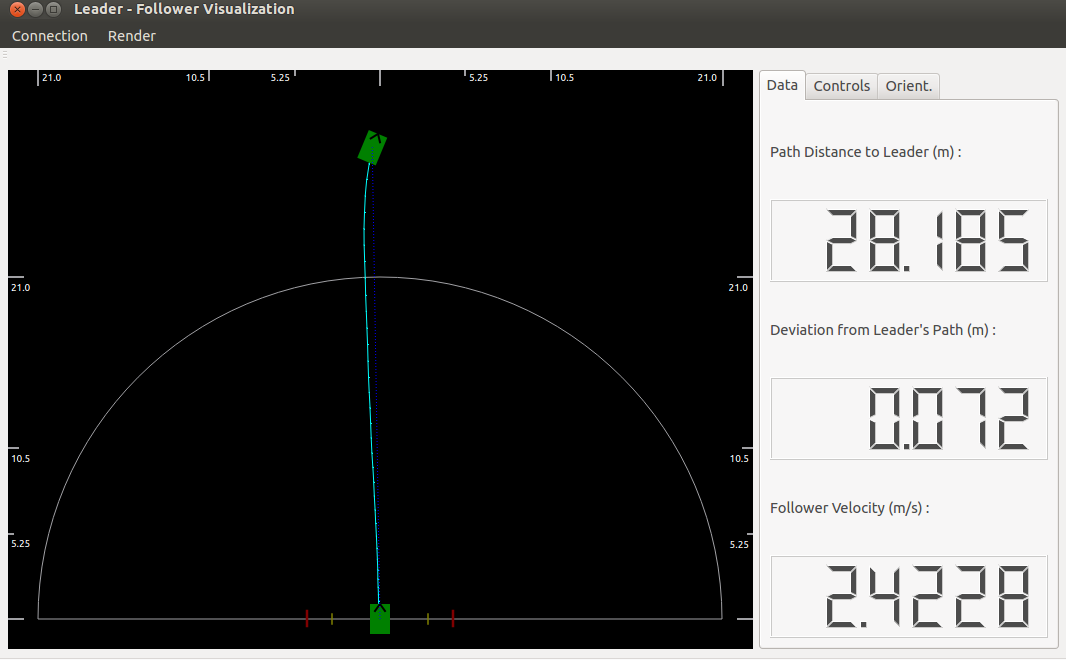
\includegraphics[width=5in]{./figs/final_design_data.png}
    \caption{Final monolithic design --- driver view} \label{fig:finaldesdriv_monolith}
\end{figure}

% the option screen
\begin{figure}[ht] \centering
    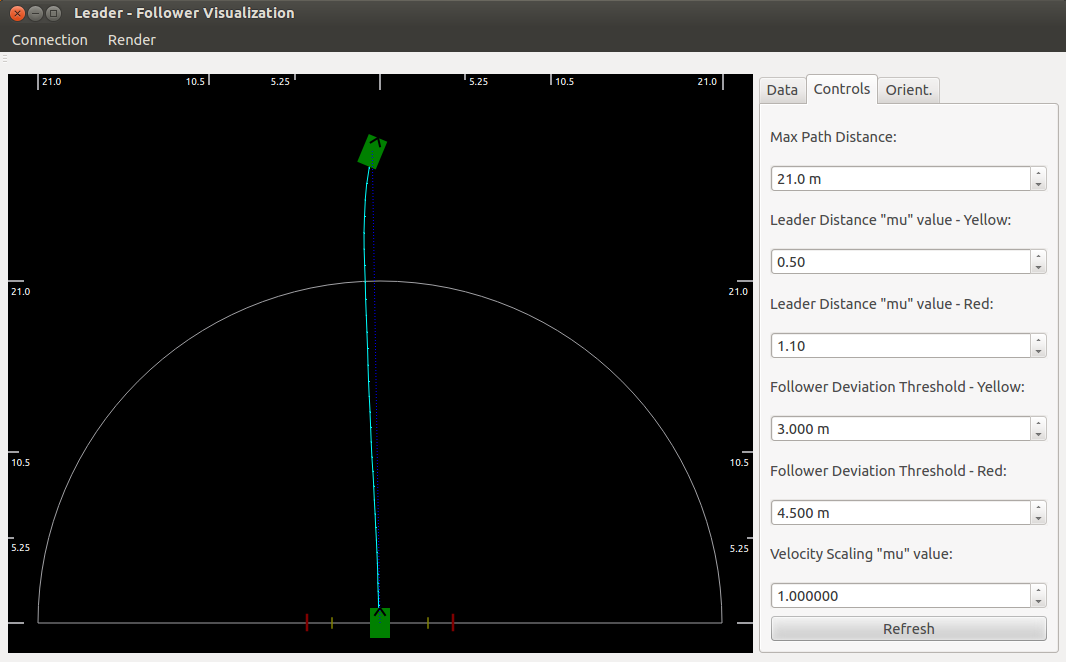
\includegraphics[width=5in]{./figs/final_design_opts.png}
    \caption{Final monolithic design --- setting of operational parameters} \label{fig:finaldesopts}
\end{figure}

%% options screen
A total of five operational parameters may be varied using the screen depicted in Figure \ref{fig:finaldesopts}, four of which are those mentioned in Sec. \ref{sec:guicalc}: the two lateral deviation thresholds and the two following distance $\mu$ thresholds. Since no global coordinates are used here, screen size is directly proportional to east and north distances in meters by some scalar value. To determine this ratio, the user inputs a maximum range distance value corresponding to the outer radius of a range indicator semicircle displayed onscreen. The number of pixels needed to display that semicircle then determines how all other objects are scaled. Since the representions of each vehicle convey important infomation, these features are not allowed to change in size, but rather occupy a constant number of pixels determined by the size of the display device. To assist in communicating the relative lengths represented, scaling legends are placed on the left, right, and top of the black render area where graphics are displayed. The drawback to this constant maximum range display is that the leader may lie outside of it, potentially disorientating the user. However, was curtailed by adding optional functionality for automatically scaling the view screen such that the leader is always within the range semicircle. When the option to always display the lead vehicle is enabled, the user-input maximum range distance becomes the minimum value, and whenever the direct distance to the follower exceeds this, the screen is scaled to include it in the range semicircle. The tradeoff is that distances must be determined by reading the values on the legend.

%%%% Earth %%%%
\subsection{Google Earth GUI} \label{sec:finaldes_earth}

With the Earth-based incarnation, design goals had been changed considerably. Since the presence of satellite imagery drastically increases the amount of  visual stimuli, it was decided that the user should be able to enter view-only mode and be rid of any objects designed for input once operational parameters had been settled upon. To this end, the command interface was liberated from the central display screen and forms its own window outside the Earth environment. The command interface backend remains as the object carrying out all mathematical calculations. This makes it simpler to get the current values of any operational parameters needed wihout incurring additional overhead since their values are also attributes of the same object. One valuable feature addition was the ability to focus the satellite camera directly above either vehicle and track its motion. Should one wish to track both, functionality is in place to track the point in space halfway between each. Should they move too far apart to view, zoom controls allow refocusing the image.

%%%% alerts - TODO get a shot with the data screen
\begin{figure}[ht] \centering 
    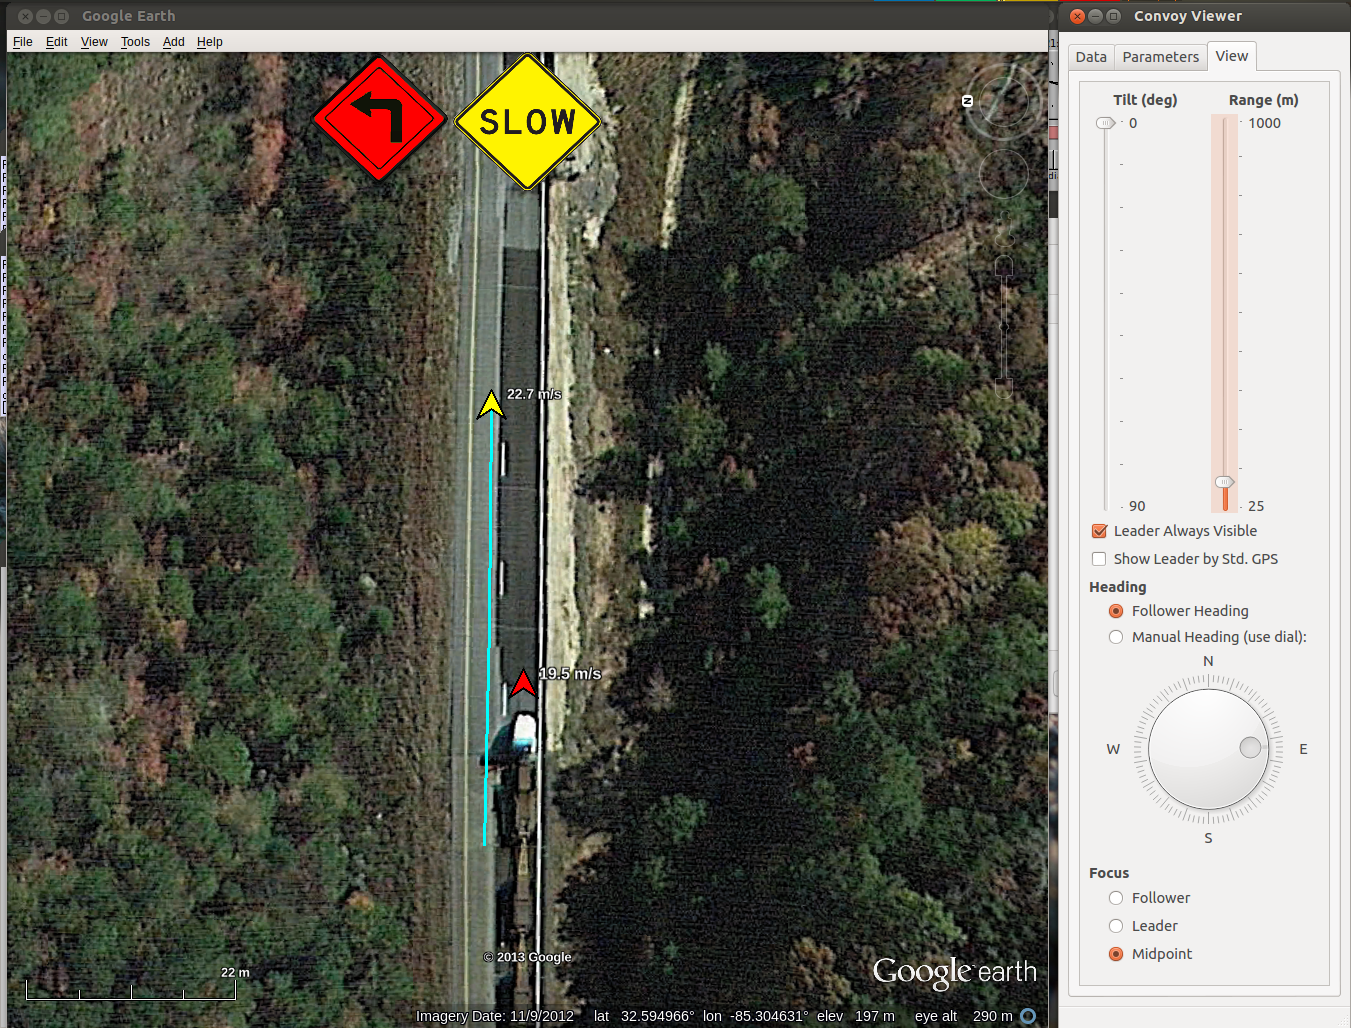
\includegraphics[width=5in]{./figs/earth_slow.png}
    \caption{Following driver being signalled in Google Earth to correct left and slow} \label{fig:earth_dst}
\end{figure}

Figure \ref{fig:earth_dst} depicts both leader and follower on a straightaway, with the follower travelling too fast and too closely to the leader for acceptable safety limits, but within critical boundaries. As such, a yellow traffic sign depiction is presented to the driver communicating the need to reduce speed, thus increasing the separation distance. Being all the way in the wrong lane to the right of the path, the lateral deviation has passed out into a critical state, so a red traffic sign depiction is displayed which communicates to the driver the need to correct left.

% TODO Range/tilt/heading information

%%%%%%%%%%%%%%%%%%%%%%%%%%%%%%%%%%%%%%%%%%%%%%%%%%%%%%%%%%%%%%%%%%%%%%%%%%%%%%%%
%   Chapter 3
%%%%%%%%%%%%%%%%%%%%%%%%%%%%%%%%%%%%%%%%%%%%%%%%%%%%%%%%%%%%%%%%%%%%%%%%%%%%%%%%
\chapter{Experimentation}
\label{chap:exper}

%%%%%%%%%%%%%%%%%%%%%%%%
% Hardware Setup Section
\section{Hardware Setup} \label{sec:hardware}

All experimental data was taken using Novatel Propak v3 GPS receivers with pinwheel antennas, identical to those used in \cite{scottthesis}. All positioning computation was conducted on an Apple MacBook Pro Laptop running Ubuntu Linux 12.04.1 in a Parallels virtual machine which was located in the rearmost vehicle. This machine also hosted and displayed the GUI during all test runs. Novatel data was relayed directly from receivers in other vehicles to the positioning computer through the use of XTend-PKG $900~MHz$ radio modems operating at a power output of $1~W$ and connected via RS232-USB adapters. This eliminated the need for additional computers, which was found to introduce unacceptable latency into the system. In this manner, a single central hub was able to host the MOOS database while controlling all receivers and data flow to all position algorithms without the needing two-way radio communication for the GUI. Figure \ref{fig:hardwarelead} depicts what hardware is necessary in the leading vehicle, and Fig. \ref{fig:hardwarefoll} depicts the hardware placed in the following vehicle, within easy sight of the driver.

\begin{figure}[ht] \centering
    \begin{minipage}[b]{0.45\linewidth} \centering 
        \includegraphics[width=\textwidth]{./figs/driver_view.jpg}
        \caption{GUI as presented to the driver} \label{fig:driverview}
    \end{minipage}
    \hspace{0.5cm}
    \begin{minipage}[b]{0.45\linewidth} \centering
        \includegraphics[width=\textwidth]{./figs/foll_hardware.jpg}
        \caption{Follower interior hardware} \label{fig:hardwarefoll}
    \end{minipage}
\end{figure}

% data collection
The stream of available data may be divided into two categories: raw GPS measurements used to compute a relative path online, and the measurements coming either the receiver or DAF algorithm which is displayed on-screen. When conducting experimental trials for formal analysis, the latter is recorded in order to capture exactly what was displayed to the following driver and examine their performance. The former is excluded in order to reduce the volume of data throughput and increase computing efficiency, as following distance and lateral path deviation are derived from the relative path and follower velocity alone. However, during the develop-test-refine cycle, the inverse is true; raw GPS measurements alone are recorded (again, neglecting other data for efficiency). This is then replayed to simulate online operation as algorithms are tuned.

\begin{figure}[ht] \centering
    \begin{minipage}[b]{0.45\linewidth} \centering 
        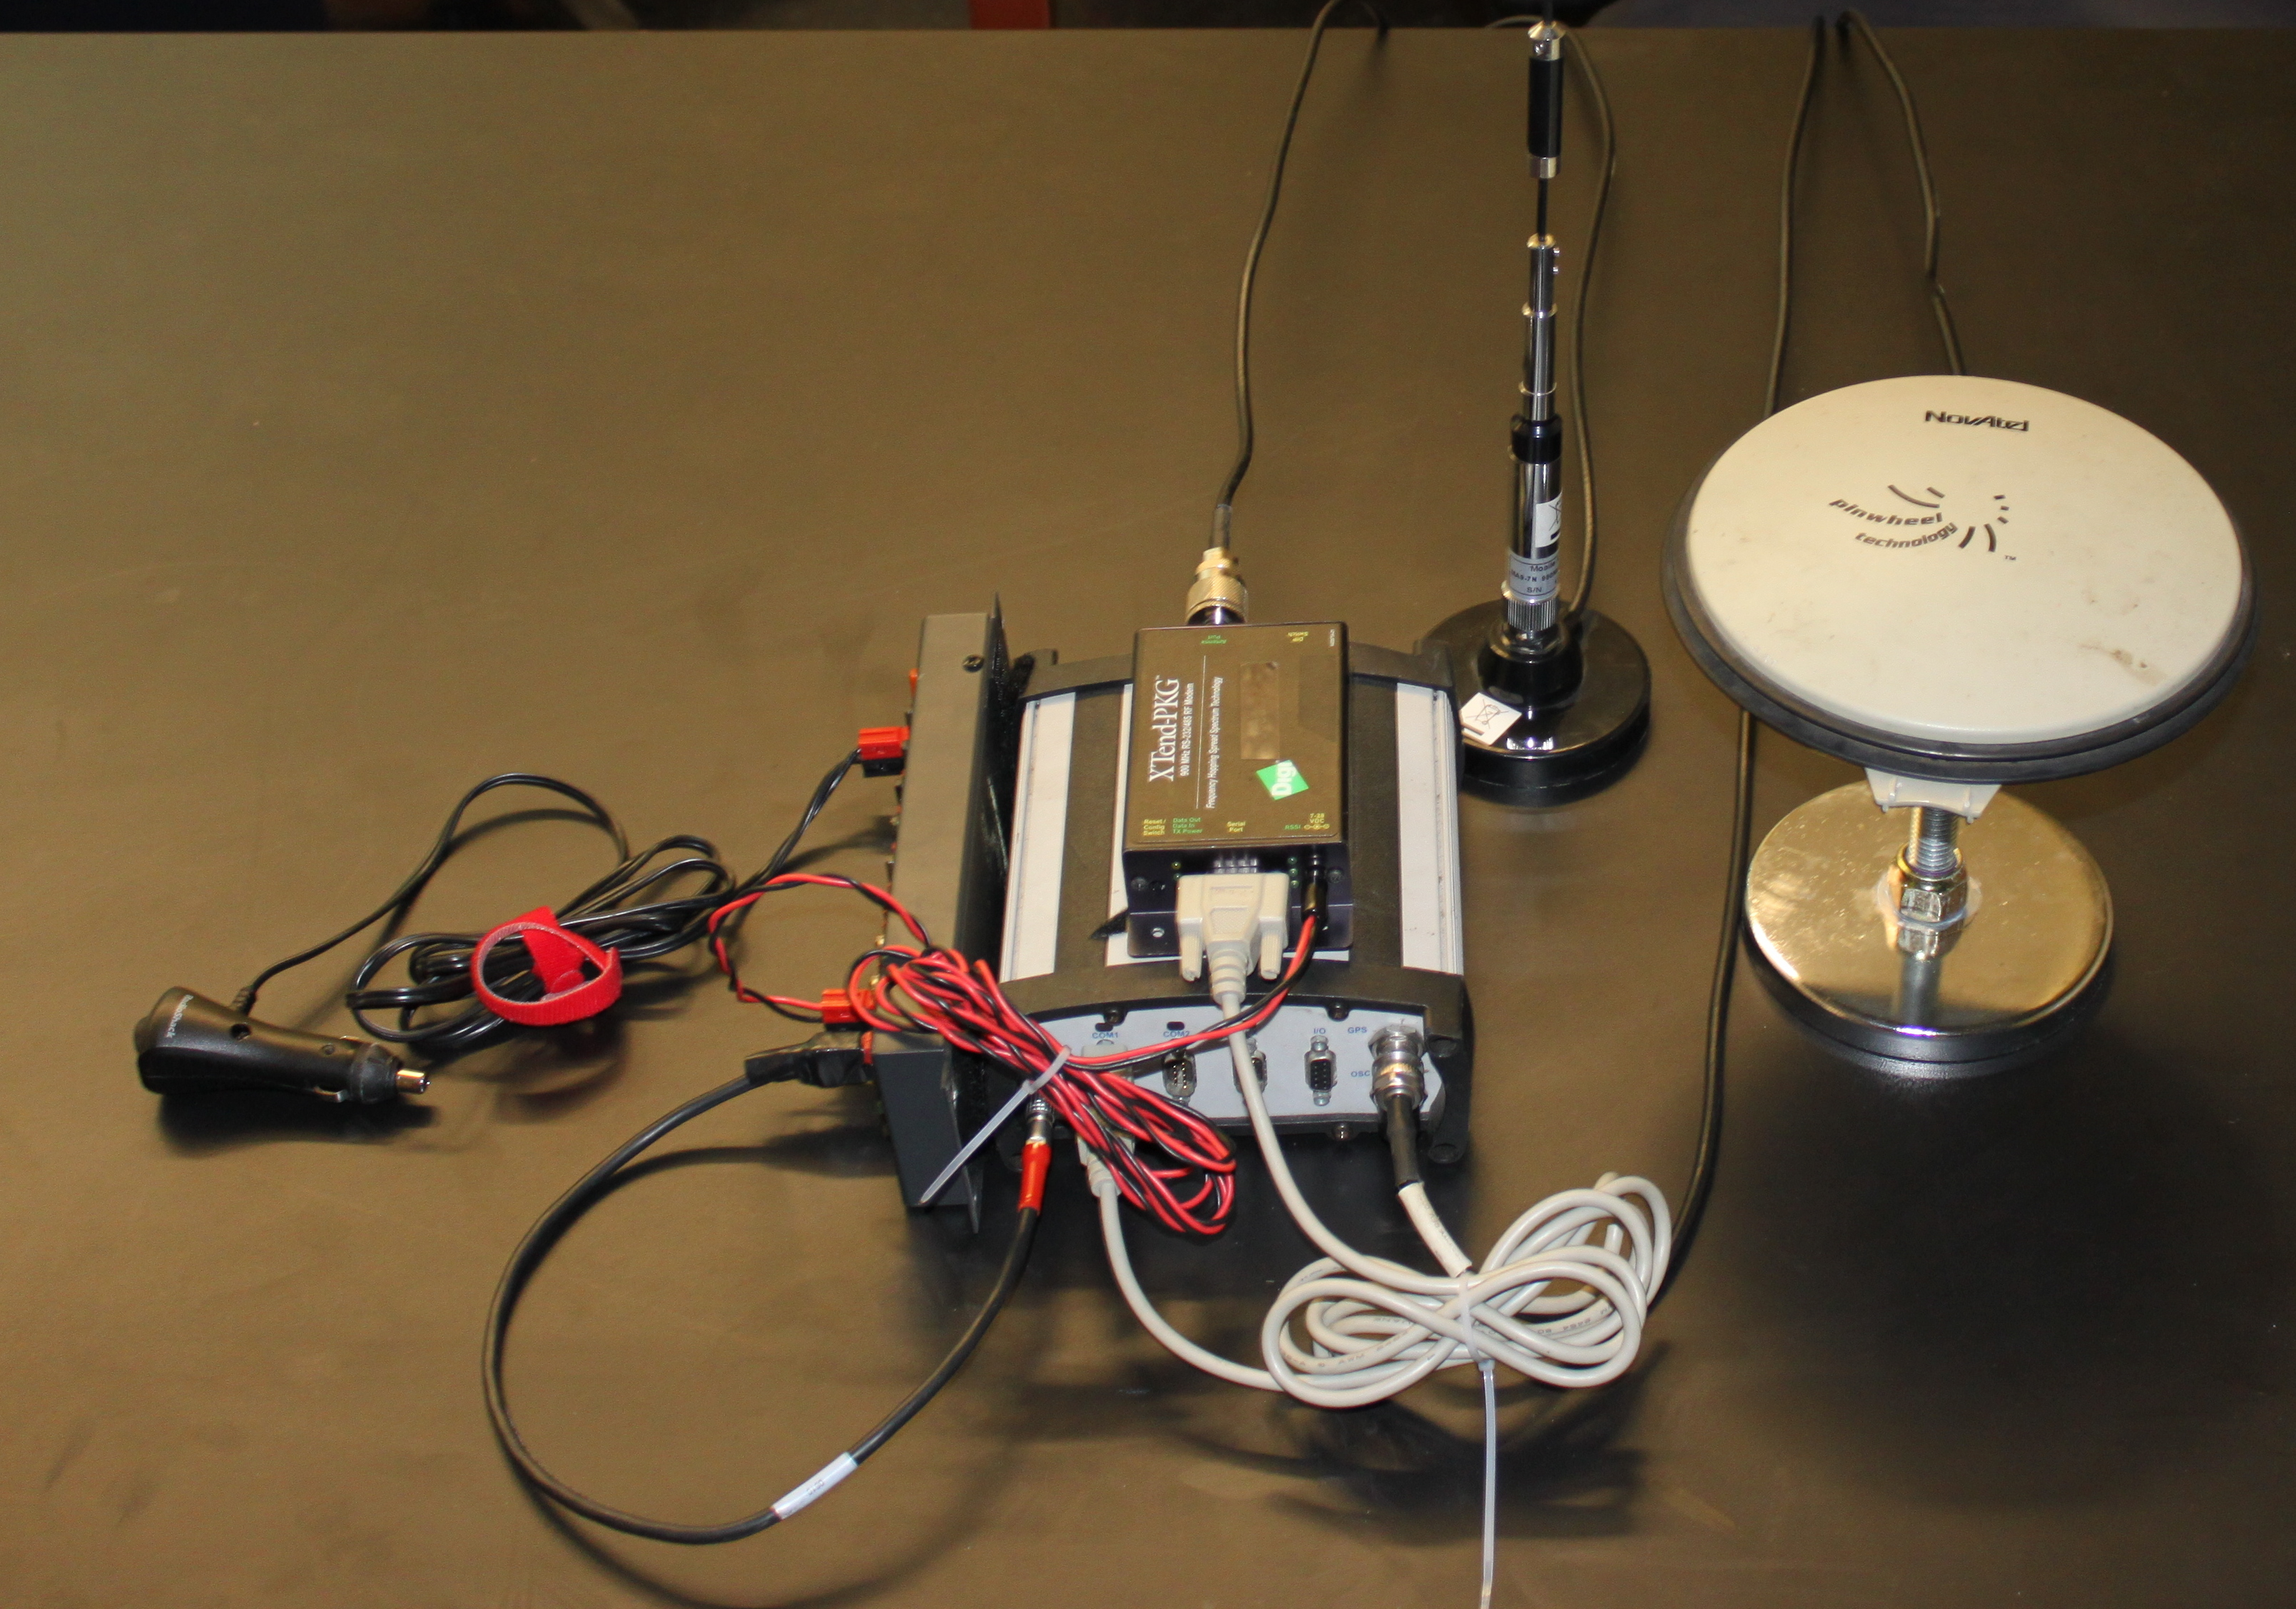
\includegraphics[width=\textwidth]{./figs/lead_hardware.jpg}
        \caption{Equipment used in the leading vehicle} \label{fig:hardwarelead}
    \end{minipage}
    \hspace{0.5cm}
    \begin{minipage}[b]{0.45\linewidth} \centering
        \includegraphics[width=\textwidth]{./figs/foll_antennae.jpg} 
        \caption{Antennaes as placed on either vehicle} \label{fig:antennaefoll}
    \end{minipage}
\end{figure}


%%%%%%%%%%%%%%%%%%%%%%%%%%%
% What tests were performed
\section{Testing} \label{sec:test}
In order to formally quantify the ability of the tools developed in Chap. \ref{chap:gui} to assist convoy drivers in the target circumstances, three tests were devised: a lane change replication test, a target spacing maintenance test, and a limited visibility test. These were also conducted to compare and contrast the two approaches embodied by each GUI. Since the tools developed before are designed for a single leader/follower pair, as few as two vehicles can be used as a convoy. Until Chap \ref{chap:errprop}, this configuration will be used.

%%%% Lane change replication
\subsection{Lane Change Replication Test} \label{sec:lanechangetest}
In determining the usefulness of any tool, it is highly desirable to devise a test which yields concise results that are either completely positive or negative. To this end, a maneuver common in typical roadway driving, the lane change, was used in a situation in which the maneuver could be replicated properly or improperly to produce a binary result. This test takes place on the National Center for Asphalt Technology (NCAT) test track in Opelika, AL, which is a two lane, 1.7 mile oval oval with turns comparable to those found on an interstate highway. The leader rounds a $180^\circ$ turn and upon exiting makes a lane change between any of six cones spaced $10m$ apart along the center stripe at the start of the straightaway. This event is visually obscured from the following driver, who has no foreknowledge of which cone pair will be chosen, so there is a $20\%$ chance of choosing the correct pair simply by guessing. This iteration of this test was performed twice, once with the monolithic GUI and once with the Earth-based GUI. No control run is needed, since a cumulative success rate across all iteration above $20\%$ represents an improvement from driving without navigation assistance. A range of highway driving speeds from 30 mph to 70 mph was used, and forward spacing was not examined except to ensure that it was large enough for the aforementioned visual obstruction.

This focused on aiding a driver in conditions where visibility is totally denied, as foliage and terrain features lie between the two vehicle during the moment of interest. Sensor and display frequencies will play a large role in this outcome. If information is updated with real time interpolation, a delay of at least one timestep (not including calculation time) is present, meaning that a worst-case GPS output frequency of 1.0 Hz will result 1.0 s data lag. For a following vehicle is travelling at 55 mph (24.5872 m/s), a 24.5872 m discrepancy between the path satellite imagery and the actual path. The impact of that behavior is one thing being examined in the lane change replication test. For the monolithic GUI, this test will show whether the range scaling indicators adequately convey distance information so that a driver can determine where to turn, when the interpolation functionality is disabled for rapid updating. The results are outlined in Sec \ref{sec:lanechangetestresults}

%%%% Target Spacing Test
\subsection{Precision Following Test} \label{sec:targetspacingtest}
The lane change replication test one example of implementing the path duplication tool, but does not produce the detailed results necessary for a formal conclusion favoring the usefulness of one GUI over the other. Centimeter-level measurements are available, so it is of great interest to determine whether either tools enables a convoy driver to carry out the following task with this same level of precision. The precision following test begins and ends with both vehicles parked atop the center stripe of the NCAT test track. The lead vehicle accelerates to approximately 45 mph then begins a sinusoidal path with a mean about the center stripe, a period of approximately 10 s, and an amplitude of which puts the wheels of the lead vehicle upon the outermost lane marking at the peaks. Once reaching 45 mph, the magnitude of the leader's ground plane velocity vector will vary according to position on the track. Along the two 180$^\circ$ turns it will be approximately 45 mph, and along the straightaways it will be approximately 65 mph. Throughout the test, the following driver is attempting to maintain a inter-vehicular spacing as low as possible without incurring any distance alerts, and accumulate as little deviation over time as possible. 
This test primarily focused on distinguishing which GUI best provided aid in path duplication; for a comparative analysis, the test was conducted with the aid of each GUI individually, then without any assistance information at all. The results are outlined in Sec. \ref{sec:precisionfollowingresults}

% %%%% Circuit Around NCAT
% \subsection{Varied Driving Test} \label{sec:variedtest}
% The above tests represent very specific scenarii that, while examining situations which commonly arise in convoy driving, did not fully cover the full range of behaviors which are being aided.  A singular test was desired which would at once examine all aspects of the graphical tool and produce broad results over multiple driving scenarii. A route around the NCAT facility was devised which included non-lane driving in environments with plenty of visual references, as well as those without. The skidpad portion of this test is an environment with no visual landmarks by which to localize the leader, as it is a flat, open expanse of asphalt, and the parking lot portion contains many visual reference points. Analyzing performance when transitioning from one environment into the other will show how this effects performance. The follower is instructed to maintain a distance as close as possible to the leader without triggering a warning or critical alert for path spacing. To examine visibility-limited performance, the test was conducted during both day- and night-time. A satellite image detailing the route taken for this test is shown in Fig. \ref{fig:variedtestroute}, and the results thereof are outlined in Sec. \ref{sec:variedtestresults}

% \begin{figure}[ht] \centering \label{fig:variedtestroute}
%     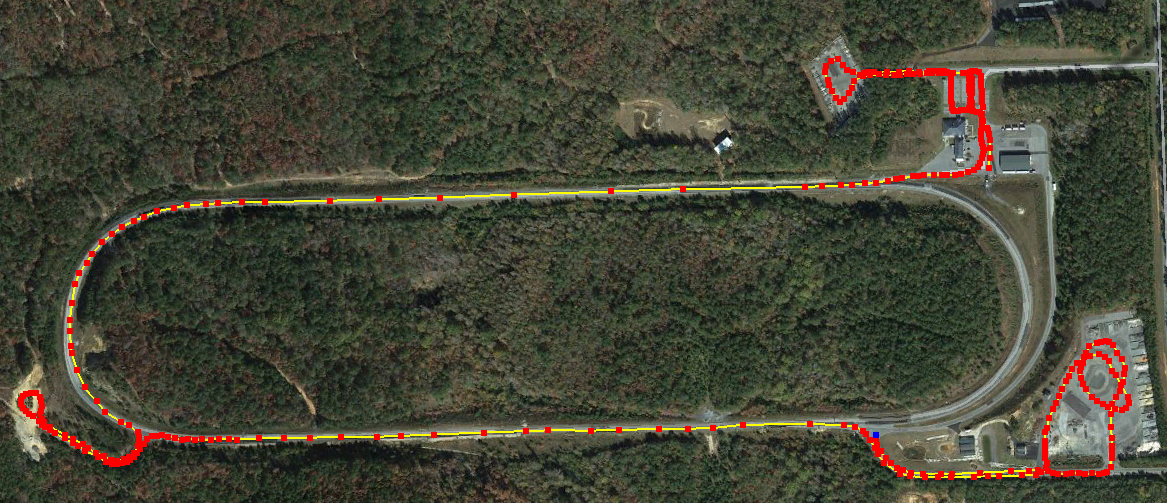
\includegraphics[width=5in]{./figs/varied_test_route.png}
%     \caption{Route taken for the varied driving test}
% \end{figure}


%%%%%%%%%%%%%%%%%
% Results section
\section{Results} \label{sec:results}

%%%%% Lane Change between Cones
\subsection{Lane Change Replication Test Results} \label{sec:lanechangetestresults}

\begin{figure}[ht] \caption{Results from all runs of the lane change replication test} \centering \label{fig:lanechangeresults}
    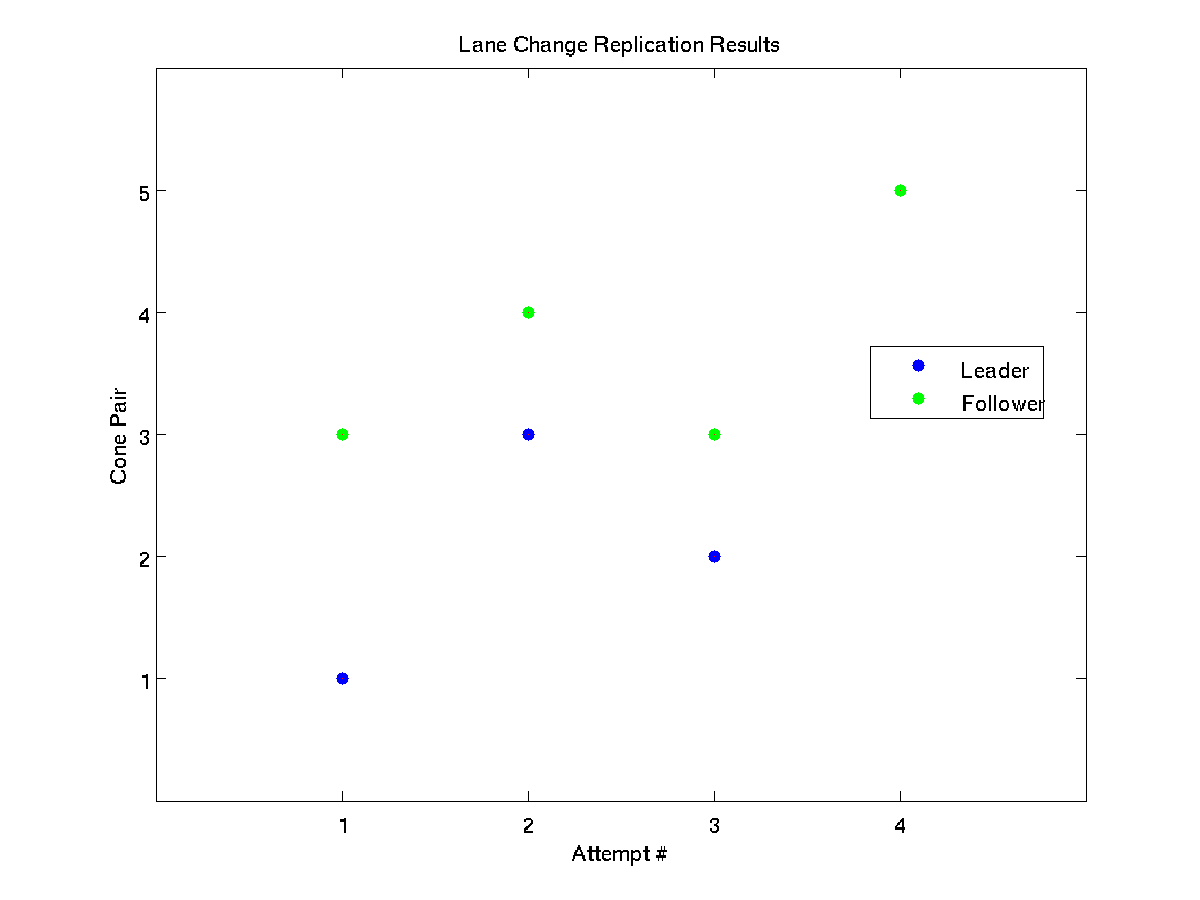
\includegraphics[width=4in]{./figs/lane_change_results.png}
\end{figure}

Figure \ref{fig:lanechangeresults} shows the results of all runs of the lane change replication test.

It is plain to see that in every instance where a lane change was made between the improper cone pair, the follower changed lanes later than did the leader. This is attributed to latency existing in the combined system from calculation and driver reaction.


%%%%% Follow the Path around the track
\subsection{Precision Following Test Results} \label{sec:precisionfollowingresults}

\begin{figure}[ht] \centering \label{fig:precisionresults_earth}
    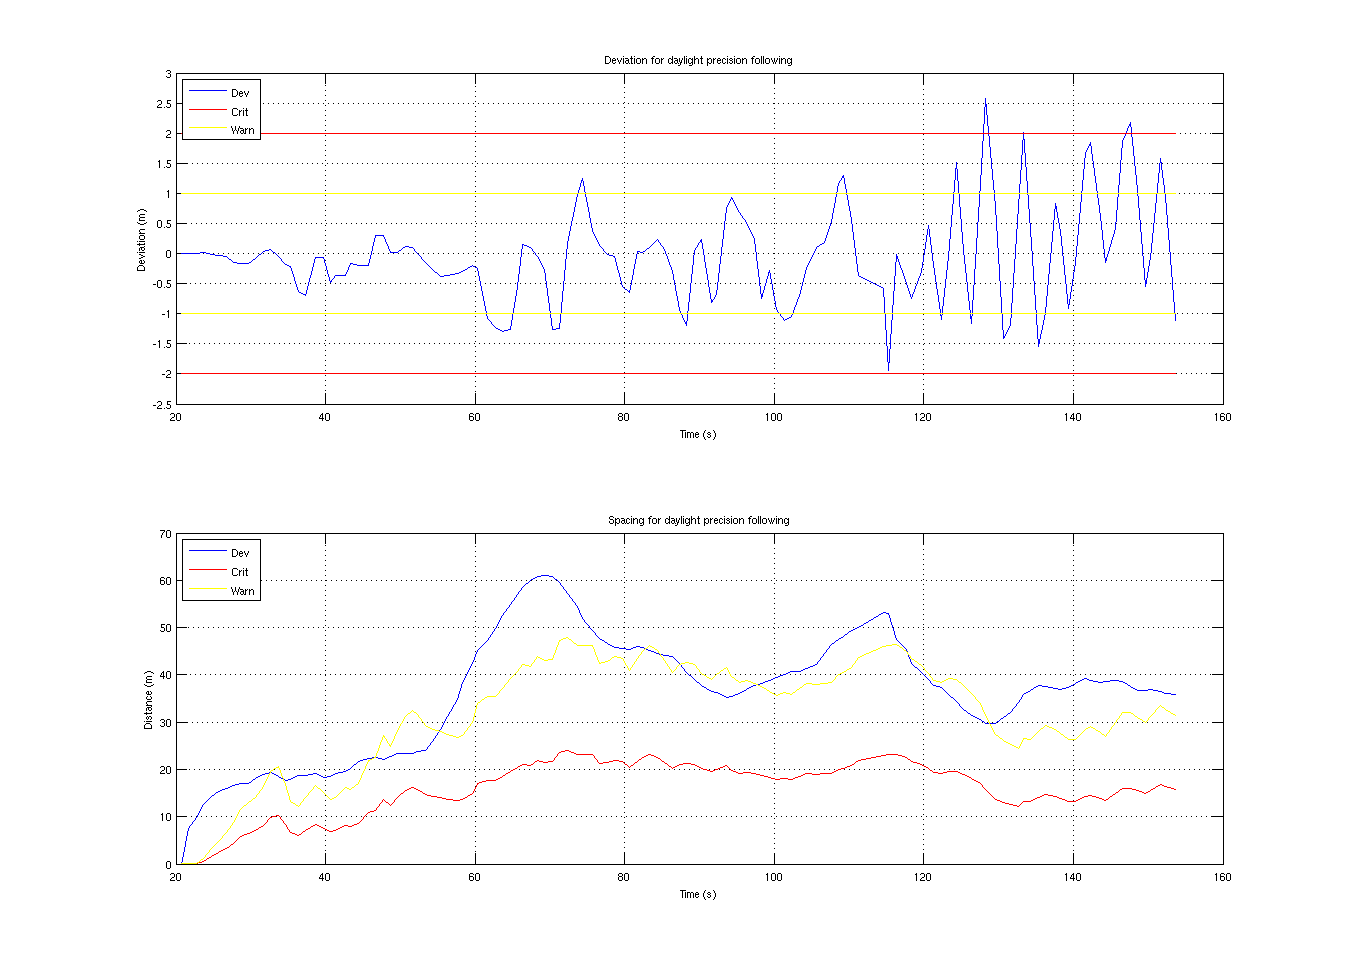
\includegraphics[width=5in]{./figs/dst_dev_earth_tracklap.png}
    \caption{Best run of the precision following test using Earth GUI}
\end{figure}

\begin{figure}[ht] \centering \label{fig:precisionresults_monolith}
    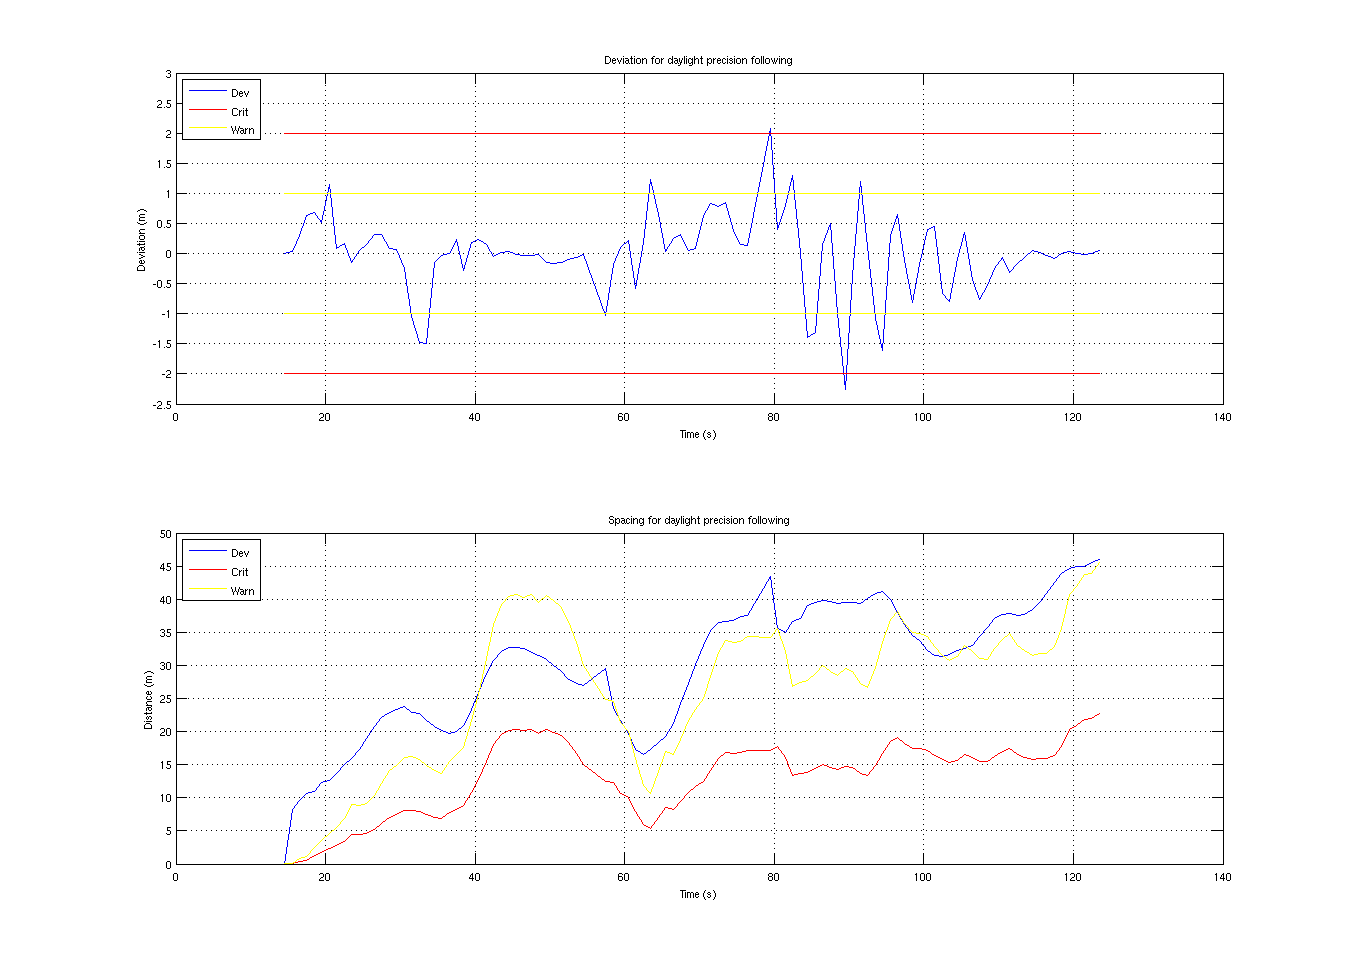
\includegraphics[width=5in]{./figs/dst_dev_monolith_tracklap.png}
    \caption{Best run of the precision following test using monolith GUI}
\end{figure}

Shown in Figs. \ref{fig:precisionresults_earth} \ref{fig:precisionresults_monolith} are the best of all runs of the precision following test. 

When at any point a path is uncalculable, due to satellite outage, outlying values, course errors, or other errors, the path reported is of length one (a single point at the position of the leader). When this occurs, the following distance becomes 0.0, and these instances are ignored in tabulation of the following distance score.





%%%%%%%%%%%%%%%%%%%%%%%%%%%%%%%%%%%%%%%%%%%%%%%%%%%%%%%%%%%%%%%%%%%%%%%%%%%%%%%%
%   Chapter 4
%%%%%%%%%%%%%%%%%%%%%%%%%%%%%%%%%%%%%%%%%%%%%%%%%%%%%%%%%%%%%%%%%%%%%%%%%%%%%%%%
\chapter{Error Propagation in Convoys} \label{chap:errprop}

\section{Introduction} \label{sec:errintro}

% RPV diagram
\begin{figure}[ht] \centering \label{fig:rpvs}
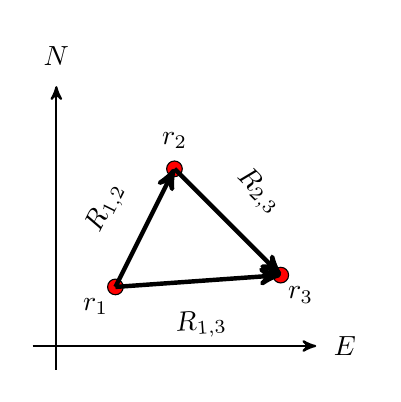
\begin{tikzpicture}[
        scale=3,
        axis/.style={thick, ->, >=stealth'},
        vector/.style={ultra thick, ->, >=stealth'},
        every node/.style={circle, color=black}
    ]
    \draw[axis] (-0.1,0) -- (1.1,0) node(xline)[right] {$E$};
    \draw[axis] (0,-0.1) -- (0,1.1) node(yline)[above] {$N$};
    % points
    \coordinate (a) at (0.25,0.25);
    \coordinate (b) at (0.5,0.75);
    \coordinate (c) at (0.95,0.3);
    \foreach \x in {a,b,c} {
        \node[draw,circle,inner sep=2pt,fill=red] at (\x) {};
    }
    \node [below left] at (a) {$r_1$};
    \node [above] at (b) {$r_2$};
    \node [below right] at (c) {$r_3$};
    % arrows
    \draw[vector] (a) -- (b) node [pos=0.5, sloped, above] {$R_{1,2}$};
    \draw[vector] (b) -- (c) node [pos=0.5, sloped, above] {$R_{2,3}$};
    \draw[vector] (a) -- (c) node [pos=0.5, sloped, below] {$R_{1,3}$};
\end{tikzpicture}
\caption{RPVs used in investigation}
\end{figure}

%%%%% Problem definition
At its simplest, this chapter will examine errors in an RPV resultant from the summantion of multiple intermediate RPVs as compared to an RPV between two points directly. That is, when using DRTK to compute RPVs, how do the errors of $~R_{1,2}+R_{2,3}~$  compare to those of $~R_{1,3}~$? To establish a nomenclature, $R_1$ shall be thought of as a convoy leader, $R_2$ as an intermediate vehicle, and $R_3$ as a following vehicle.


\section{Experimentation}
A one hour data set was taken with three antennas completely static --- meaning a fixed baseline --- 

A half hour data set was recorded with all three antennas at the same baseline as the set described before, but the vehicle on which all three were mounted was driven in chaotic patterns at speeds between $4.5~m/s$ and $13.5~m/s$ in a GPS-benign environment.


\section{Results}

% Fixed baseline Static
\begin{figure}[ht] \centering \label{fig:fixed_static_err_rpv}
    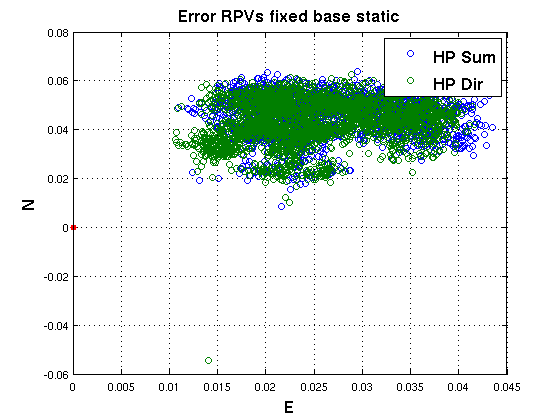
\includegraphics[width=6.5in]{./figs/fixed_static_error_rpv.png}
    \caption{}
\end{figure}

\begin{figure}[ht] \centering \label{fig:fixed_static_err_mag}
    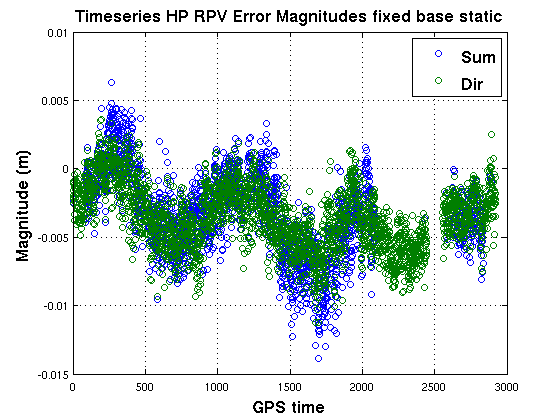
\includegraphics[width=6.5in]{./figs/fixed_static_err_mags.png}
    \caption{}
\end{figure}

% Fixed baseline Dynamic
\begin{figure}[ht] \centering \label{fig:fixed_dynamic_err_rpv}
    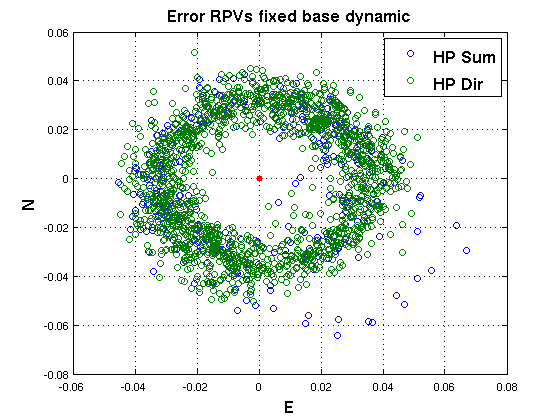
\includegraphics[width=6.5in]{./figs/fixed_dynamic_error_rpv.png}
    \caption{}
\end{figure}

\begin{figure}[ht] \centering \label{fig:fixed_dynamic_err_mag}
    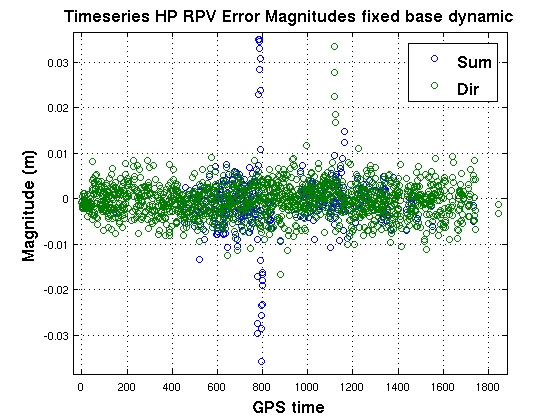
\includegraphics[width=6.5in]{./figs/fixed_dynamic_err_mags.png}
    \caption{}
\end{figure}



% Results table
\begin{table}[htbp] \caption{Statistical Comparison} \centering
\begin{tabular}{r||c|c} \hline
                & Fixed Base, Static  &  Fixed Base, Dynamic \\
    \hline \hline
    Variance, mag of errors & & \\
        Sum (mm): & 0.008 & 0.023 \\
        Dir (mm): & 0.005 & 0.014 \\ \hline
    RMS value of mag errors & & \\
        Sum (mm): & 3.854 & 3.162 \\
        Dir (mm): & 3.684 & 2.810 \\ \hline
\end{tabular} \label{tab:turb_interp} \end{table}




%%%%%%%%%%%%%%%%%%%%%%%%%%%%%%%%%%%%%%%%%%%%%%%%%%%%%%%%%%%%%%%%%%%%%%%%%%%%%%%%
%   Chapter 5
%%%%%%%%%%%%%%%%%%%%%%%%%%%%%%%%%%%%%%%%%%%%%%%%%%%%%%%%%%%%%%%%%%%%%%%%%%%%%%%%
\chapter{Conclusion} \label{chap:concl}


\section{Summary of Experimentation} \label{sec:summexper}



\section{Qualitative User Feedback} \label{sec:qual}


\section{Future Work} \label{sec:future}


%%%%%%%%%%%%%%%%%%%%%%%%%%%%%%%%%%%%%%%%%%%%%%%%%%%%%%%%%%%%%%%%%%%%%%%%%%%%%%%%
%   Bib
%%%%%%%%%%%%%%%%%%%%%%%%%%%%%%%%%%%%%%%%%%%%%%%%%%%%%%%%%%%%%%%%%%%%%%%%%%%%%%%%
\bibliographystyle{asmems4}
\bibliography{thesis}

\nocite{travisdiss}
\nocite{travisshort}
\nocite{calgary}

% \bibitem{platoon} M. E. Cannon, C. Basnayake, S. Syed, and G. Lachapelle. ``Precise gps sensor subsystem for Vehicle Platoon  Control." In Proceedings of ION GPS/GNSS 2003 Conference. pp 213-224, 2003.

\end{document}